\documentclass[a4paper]{article}
\usepackage[hmargin=1in, vmargin=1in]{geometry}
\usepackage{makeidx}
\usepackage{fancyhdr}
\pagestyle{fancy}
\usepackage[pdftex]{graphicx}
\usepackage{amsmath}
\usepackage{amssymb}
\usepackage{listings}
\usepackage{natbib}
%\makeindex
\begin{document}
\begin{center}
\title{Transformation dreidimensionaler Koordinaten in zweidimensionale Koordinaten (German Version)}\\
\author{Edward Gerhold}
Transformation dreidimensionaler Koordinaten in zweidimensionale Koordinaten (German version)
\date{\today}
\maketitle


Deutsche Version 0.0.98 von 0.1.0\\

\end{center} 

\tableofcontents\\

\section{Einleitung}

Auf einem Blatt Papier sehen sie drei Koordinatenachsen in drei Richtungen in den Raum zeigen.
In der Realit\"at sind diese Vektoren zweidimensional. Denn sie zeigen in drei Richtungen auf
dem Papier, und nicht in den reellen Raum.\\

\begin{figure}[ht]
\label{ijksystem}
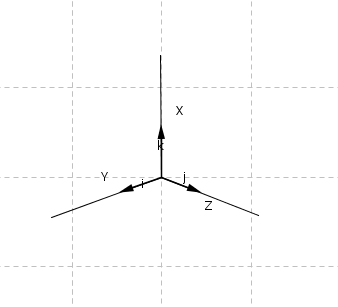
\includegraphics[scale=2]{ijksystem.png}\\
\caption{Bild eines rechtsh\"andigen Koordinatensystems mit ijk-Basisvektoren auf den Achsen, in drei dimensionen zeigend. Schauen sie in \cite{Corral1} f\"ur eine Einf\"uhrung.}
\end{figure}

In diesem Dokument entwerfen wir ein $\mathbb{R}^{2\times{3}}$ Koordinatensystem um 3-D Punkte in 2-D Punkte umzuwandeln.
Mit den Kosinus- und Sinusfunktionen rechnen wir f\"ur die horizontale und die vertikale Verschiebung des Punktes je drei Terme
der Achsvektoren mit den drei Koordinaten zusammen.\\

\textbf{Was wir in diesem Dokument machen werden.}

\begin{enumerate}
\item Winkel ausw\"ahlen f\"ur unserer Koordinatenachsen 
\item Einheiten der Achsen ausw\"ahlen oder sich f\"ur $1$ entscheiden.
\item Aufschreiben der drei zweidimensionalen Achsvektoren des Koordinatensystems.
\item Zusammenbauen der Achsen zu einer Matrix, einer Funktion oder Einsetzen anstelle einer Basis.
\item Lesen des JavaScript Codes der Transformation, der zwei Zeilen umfasst. Je eine f\"ur $x$
\item Read other versions of the transformation, with functions, for example.
\item Derive the generic case of transforming coordinate systems down to the plane.

\end{enumerate}

%\chapter{1}

\section{Entwurf eines $\mathbb{R}^{2\times{3}}$ Koordinatensystems f\"ur unsere Koordinatentransformation vom $\mathbb{R}^{3}$ auf den $\mathbb{R}^{2}$}

In der englischen Version schreibe ich alles etwas anders. Diese deutsche Fassung ist speziell neu angefangen und ich verfolge das
Ziel, mich auch etwas k\"urzer zu fassen. Mathematik, die ich in der deutschen Fassung auslassen werde, ist aber problemlos in der
englischen Version zu verfolgen. Wer das rechnen kann, kann bestimmt auch ein wenig Englisch und versteht auch deutsches Englisch.

\section{Definitionen}

\subsection{Koordinatensystem}
\subsubsection{Links- und rechts}
Ein linksh\"andiges Koordinatensystem auf der Ebene hat die dritte Achse zwischen den beiden normalen Achsen in die gleiche Richtung zeigend.

\begin{figure}
\caption{Ein linksh\"andiges Koordinatensystem}
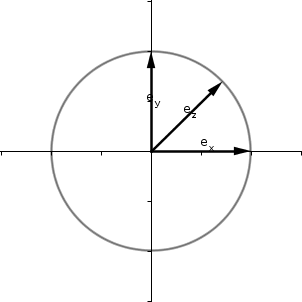
\includegraphics[scale=0.5]{lefthand45.png}
\end{figure}

Bei einem rechtsh\"andigen Koordinatensystem auf der Ebene zeigt die dritte Achse in die entgegengesetzte Richtung.

\begin{figure}
\caption{Ein rechtsh\"andiges Koordinatensystem}
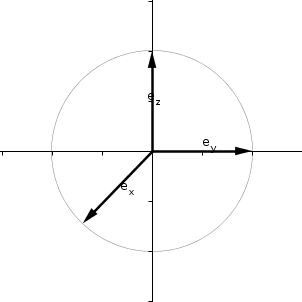
\includegraphics[scale=0.5]{righthand45.png}
\end{figure}

\subsubsection{Einheitskreis}

Der Einfachheit halber kann man die drei Achsen am Einheitskreis ausrichten. Dazu bedienen wir uns gleich einer hilfreichen Formel aus dem Polarkoordinatensystem.

\begin{displaymath}
	(x,y) := (r \cos \varphi, r \sin \varphi)
\end{displaymath}

$(x,y)$ stellen die Spitze eines Ortsvektors aus Zentrum des Koordinatensystems dar. Wenn wir drei Achsen haben wollen, sollten wir
uns drei solche Vektoren erzeugen. Das werden wir auch gleich tun. 


\subsection{Winkel der Achsen}

Die Achsen werden von der horizontalen x-Achse des zweidimensionalen Bilds gegen den Uhrzeigersinn gez\"ahlt. Da wir drei Achsen haben, brauchen wir auch drei Winkel.

\begin{displaymath}
	\varphi_n := \{ \varphi_x, \varphi_y, \varphi_z | \mbox{ die Winkel der drei Achsen}\}
\end{displaymath}

Die Winkel kann man selbst in Grad oder Radians festlegen. Die Programmiersprache JavaScript zum Beispiel nimmt, f\"ur die Funktionen Kosinus und Sinus die Winkel, in Radians an. Die sind mit einer einfachen Formel berechenbar.

\begin{displaymath}
	\mbox{rad}(\mbox{deg}) := \frac{\pi}{180} \times \mbox{deg}
\end{displaymath}

\begin{displaymath}
	\mbox{deg}(\mbox{rad}) := \frac{180}{\pi} \times \mbox{rad}
\end{displaymath}

\subsection{Einheit der Achsen}
\subsubsection{Der r-Wert der Achsen}

\begin{displaymath}
	r_n := \{ r_x , r_y , r_z | \mbox{ die Einheit jeder der drei Achsen}\}
\end{displaymath}



\subsubsection{Mathematische Vorsicht mit dem r-Wert}

Der r-Wert verkompliziert die Berechnungen und Absch\"atzungen nat\"urlich, weil die Koordinaten mit multipliziert werden. \\

Wenn man bewegte Bilder produzieren will, sollte der r-Wert grundsaetzlich gleich auf allen Achsen sein, weil Rotationen und Translationen sonst daneben gehen, da die Punkte dann pl\"otzlich ihre Einheiten wechseln. Das sieht unrealistisch aus, ist aber
bei Standbildern kein Problem.\\

Die Formel verkompliziert sich bei drei verschiedenen r-Werten nat\"urlich und zum Rechnen sollte zuerst das vereinfachte Modell
herangezogen werden, wo der r-Wert auf allen drei Achsen gleich ist, oder gleich $1$ ist und komplett entf\"allt.\\

\subsection{(Basis)vektoren der Linearkombination}

Wir ben\"otigen f\"ur das Koordinatensystem drei Achsen. Jede Achse bekommt einen kanonischen Einheitsvektor. 

\begin{displaymath}
\vec{e}_n := \{ \vec{e}_x, \vec{e}_y, \vec{e}_z | \vec{e}_n = \begin{pmatrix}r_n \cos \varphi_n\\r_n \sin \varphi_n\end{pmatrix}, \mbox{ die drei Achsen des Koordinatensystems }\}
\end{displaymath}

Wenn der r-Wert gleich $1$ ist, haben diese Vektoren gleich normalisierte Einheitsl\"ange im Sinne der Orthonormalbasis. Der Unterschied zur Orthonormalbasis ist, dass wir mindestens eine linear abh\"angige Achse haben. Je nach Arrangement um den Kreis k\"onnen dabei bis zu drei linear abh\"angige Achsen entstehen, in Bezug zur 2-D Standardbasis $\begin{pmatrix}1&0\\0&1\end{pmatrix}$ auf die das Ergebnis abgebildet wird.\\


\section{Transformationswerkzeuge}

In diesem Kapitel stelle ich dann vor, wie man die Transformation durchf\"uhrt.

\subsection{Anstelle der Basis}

Wir definieren mit $x\vec{i}+y\vec{j}+z\vec{k}$ in der Regel einen Vektor mit einer 3x3 Basis. Man kann die 2x3 Basis anstelle der 3x3 Basis einsetzen und erh\"alt eine saubere Orthogonalprojektion.

\begin{displaymath}
x\vec{e}_{x} + y\vec{e}_{y} + z\vec{e}_{z} = \vec{w} 
\end{displaymath}



\subsection{Funktional}

Die Funktion nimmt einen Vektor mit drei Koordinaten an und gibt einen Vektor mit zwei Koordinaten zur\"uck. Den richtigen Punkt.

\begin{displaymath}
\vec{f}(\vec{x}) := x \begin{pmatrix}r_x \cos \varphi_x\\r_x \sin \varphi_x\end{pmatrix} +y  \begin{pmatrix}r_y \cos \varphi_y\\r_y \sin \varphi_y\end{pmatrix} +z  \begin{pmatrix}r_z \cos \varphi_z\\r_z \sin \varphi_z\end{pmatrix}
\end{displaymath}


\subsection{Matrix}

Die Multiplikation der Matrix mit einem dreidimensionalen Vektor gibt einen zweidimensionalen Vektor zur\"uck. Den richtigen Punkt.

\begin{displaymath}
\boldsymbol{A} := 
\begin{pmatrix}
r_x \cos \varphi_x&
r_y \cos \varphi_y&
r_z \cos \varphi_z\\

r_x \sin \varphi_x&
r_y \sin \varphi_y&
r_z \sin \varphi_z
\end{pmatrix}

\end{displaymath}

\section{Transformationsverhalten}

Die Transformation ist eine lineare Transformation und erf\"ullt damit die grunds\"atzlichen Bedingungen der linearen Funktionen.

\subsection{Der Ursprung wird auf den Ursprung abgebildet}

Der Nullvektor aus dem dreidimensionalen Raum $\vec{0} \in \mathbb{R}^3$ wird auf den Nullvektor im zweidimensionalen Raum abgebildet $\vec{0} \in \mathbb{R}^2$.\\

\textbf{Beweis}:
\begin{displaymath}
    \boldsymbol{A}\left(\begin{array}{1}0\\0\\0\end{array}\right)
    = \left(\begin{array}{1}0 + 0 + 0\\0 + 0 + 0\end{array}\right) 
    =\left(\begin{array}{1}0\\0\end{array}\right)
\end{displaymath}\\

\subsection{Punkte auf einer Achsen}

Punkte, die nur auf einer Achse liegen sind ein vielfaches des jeweiligen Achsenvektors.\\

\textbf{Beweis}:
\begin{displaymath}
    \boldsymbol{A}\left(\begin{array}{1}a\\0\\0\end{array}\right)
    = \left(\begin{array}{1}ar_x\cos \varphi_x + 0 + 0\\ar_x\sin \varphi_x  + 0 + 0\end{array}\right) 
    = a\vec{e}_x
\end{displaymath}

\begin{displaymath}
    \boldsymbol{A}\left(\begin{array}{1}0\\1\\0\end{array}\right)
    = \left(\begin{array}{1}0 + r_y\cos \varphi_y + 0\\0 + r_y\sin \varphi_y + 0\end{array}\right) 
    = \vec{e}_y
\end{displaymath}

\begin{displaymath}
    \boldsymbol{A}\left(\begin{array}{1}0\\0\\-b\end{array}\right)
    = \left(\begin{array}{1}0 + 0 - br_z\cos \varphi_z\\0 + 0 - br_z\sin \varphi_z\end{array}\right) 
    = -b\vec{e}_z
\end{displaymath}\\

\subsection{Skalare Multiplikation}

Es ist einfach zu zeigen, dass $\boldsymbol{A}(\lambda\vec{x}) = \lambda\boldsymbol{A}\vec{x}$. Man kann vor der Transformation oder nach der Transformation mit dem Skalar multiplizieren. Das Resultat ist identisch.\\

\textbf{Beweis}:\\
\begin{displaymath}
\begin{equation*}
\begin{align*}
\boldsymbol{A}(\lambda\vec{x}) &= \boldsymbol{A}\left(\begin{array}{1}\lambda{x}\\\lambda{y}\\\lambda{z}\end{array}\right)\\ &= \left(\begin{array}{1}\lambda{x}r_x\cos(\varphi_x) + \lambda{y}r_y\cos(\varphi_y) + \lambda{z}r_z\cos(\varphi_z)\\
\lambda{x}r_x\sin(\varphi_x) + \lambda{y}r_y\sin(\varphi_y) + \lambda{z}r_z\sin(\varphi_z)
\end{array}\right)\\
    &= \lambda\left(\begin{array}{1}xr_x\cos(\varphi_x) + yr_y\cos(\varphi_y) + zr_z\cos(\varphi_z)\\
xr_x\sin(\varphi_x) + yr_y\sin(\varphi_y) + zr_z\sin(\varphi_z)\\
\end{array}\right)\\
    &= \lambda\left(\begin{array}{1}x'\\y'\end{array}\right)\\
    &= \lambda\boldsymbol{A}\vec{x}
\end{align*}
\end{equation*}
\end{displaymath}\\


\subsection{Addition und Subtraktion}

Einfach zu zeigen ist auch, dass $\boldsymbol{A}(\vec{v} + \vec{w}) = \boldsymbol{A}\vec{v} + \boldsymbol{A}\vec{w}$. 
Man kann auch hier die Eingabevektoren vor der Umwandlung addieren, oder die Ausgabevektoren nach der Umwandlung. Die resultierende Summe ist identisch.
 
\textbf{Beweis}:\\

\begin{displaymath}
\begin{equation*}
\begin{align*}
\boldsymbol{A}\left(\begin{array}{1}x+u\\y+v\\z+w\end{array}\right) &= \left(\begin{array}{1}(x+u)r_x\cos(\varphi_x) + (y+v)r_y\cos(\varphi_y) + (z+w)r_z\cos(\varphi_z)\\
(x+u)r_x\sin(\varphi_x) + (y+v)r_y\sin(\varphi_y) + (z+w)r_z\sin(\varphi_z)\\
\end{array}\right)\\
            &= \left(\begin{array}{1}xr_x\cos(\varphi_x) + yr_y\cos(\varphi_y) + zr_z\cos(\varphi_z)\\
xr_x\sin(\varphi_x) + yr_y\sin(\varphi_y) + zr_z\sin(\varphi_z)\\
\end{array}\right) + \left(\begin{array}{1}ur_x\cos(\varphi_x) + vr_y\cos(\varphi_y) + wr_z\cos(\varphi_z)\\
ur_x\sin(\varphi_x) + vr_y\sin(\varphi_y) + wr_z\sin(\varphi_z)\\
\end{array}\right)\\    
    &= \left(\begin{array}{1}x'\\y'\end{array}\right) + \left(\begin{array}{1}u'\\v'\end{array}\right)\\
    &= \boldsymbol{A}\left(\begin{array}{1}x\\y\\z\end{array}\right) + \boldsymbol{A}\left(\begin{array}{1}u\\v\\w\end{array}\right)
\end{align*}
\end{equation*}
\end{displaymath}

\subsection{Linearit\"at}

Durch die letzten zwei Beweise ist es offensichtlich, dass die Transformation die Regeln der Linearit\"at befolgt.

\begin{displaymath}
\boldsymbol{A}(\lambda\vec{v} + \kappa\vec{w}) = \lambda\boldsymbol{A}\vec{v} + \kappa\boldsymbol{A}\vec{w} = \lambda\left(\begin{array}{1}x'\\y'\end{array}\right) + \kappa\left(\begin{array}{1}u'\\v'\end{array}\right)\\
\end{displaymath}

Auf den Beweis der Kombination beider Abschnitte verzichte ich.\\


\section{Selbst\"andigkeitserkl\"arung}

Ich habe dieses Koordinatensystem selbst entwickelt. Es ist keine Formel aus einem Buch oder einer Lehrveranstaltung.
Ob es irgendwo eine identische Formel oder eine vergleichbare Definition gibt, ist mir nicht bekannt.
Ich habe den Inhalt des Dokuments aus eigenem Ermessen zusammengestellt. Ich habe mir Gedanken zum Thema gemacht und
ausserdem Rechnungen mit Stift und Papier angefertigt. Ausserdem habe ich in Lehrb\"uchern und Veranstaltungen gebl\"attert,
um das Koordinatensystem und die definierten Variabeln und Operationen m\"oglichst gut in die reelle Mathematik einzuordnen.
Mir m\"ogen Fehler unterlaufen sein, und auch Details entgangen sein. F\"ur beides m\"ochte ich mich entschuldigen.\\


\section{Lizenz}

Der produzierte Source Code, um das Koordinatensystem und einige Abbildungen zu zeigen, ist frei f\"ur alle,
wie auch das Koordinatensystem selbst und die dazugeh\"origen Definitionen, die ich selbst angefertigt habe.
Es ist erlaubt, mir daf\"ur Anerkennung zu gew\"ahren, es ist aber nicht zwingend n\"otig, mich daf\"ur im
eigenen Projekt zu nennen. Allerdings mag auch ich keine Menschen, die diese Arbeit f\"ur ihre eigene ausgeben.\\


\begin{thebibliography}
% books

    \bibitem{Corral1} \textit{Michael Corral, Schoolcraft College},
            Vector Calculus, GNU Free Documentation License, http://mecmath.net 
    \bibitem{Corral2} \textit{Michael Corral, Schoolcraft College},
            Trigonometry, GNU Free Documentation License, http://mecmath.net
    \bibitem{Strang1} \textit{Gilbert Strang, MIT},
            Linear Algebra and it´s Applications. Fourth Edition.        
    \bibitem{Strang2} \textit{Gilbert Strang, MIT},
            Calculus. MIT OpenCourseWare Supplemental Resources. http://ocw.mit.edu    
% lecture scripts english
    \bibitem{Toplogy} \textit{ ,  },
            Lecture Script, Topology (english),
    \bibitem{Functional1} \textit{},
            Lecture Script, Functional Analysis (english),    
    \bibitem{Functional2} \textit{TODO},
            Lecture Script, 
    \bibitem{Functional3} \textit{TODO},
            Lecture Script,
% lecture scripts in german
    \bibitem{Ferus1} \textit{Dirk Ferus, TU-Berlin, em.},
            Lecture Script, Lineare Algebra 1+2, 2000, http://page.math.tu-berlin/~ferus/skripten.html
    \bibitem{Kuehn1} \textit{Franziska K\"uhn, Technische Universit\"at Dresden},
            Lecture Script, Lineare Algebra und analytische Geometrie I+II, http://fkuehn.de/download/LAAG.pdf
    \bibitem{Wittbold} \textit{Petra Wittbold, TU-berlin},  
            Lecture Script, Funktionalanalysis I,  http://www3.math.tu-berlin.de/Vorlesungen/SS09/FA1/Doc/Funkana1-SS06-08.06.09.pdf
% latex tutorials 
    \bibitem{Corral3} \textit{Michael Corral, Schoolcraft College},
            Latex Mini Tutorial, http://mecmath.net                    
    \bibitem{Jürgens,Feuerstack} \textit{Manuela J\"urgens, Thomas Feuerstack, Fernuniversit\"at Hagen},
            LaTeX, eine Einf\"uhrung und ein bisschen mehr..., a026\_latex\_einf.pdf            
    \bibitem{Rudl} \textit{Dr.Jan Rudl, Technische Universit\"at Dresden, Fachbereich Mathematik},
            Einf\"uhrung in LaTeX, LaTeX-Kurs.pdf            
\end{thebibliography}



\printindex

\end{document}

